Stadia Follows  Promotion strategy to attract more users/gamer in many different ways,
like many advertisements and hot offers. It also tries to attract developers to maintain its technology to be up to date and provide its service with everything a user needs.
we will discuss its tools in the following subsections.

\begin{figure}[h]
    \centering
    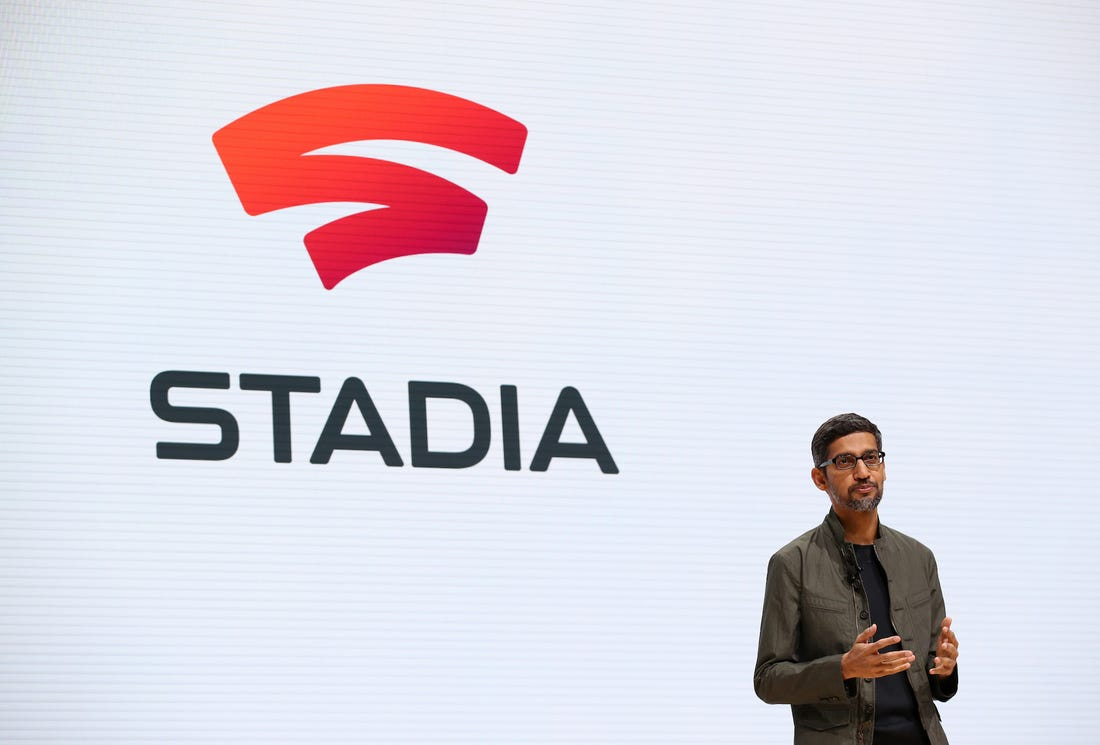
\includegraphics[width=0.8\textwidth]{images/release.jpeg}
    \caption{Stadia Release}
    \label{fig:release}
\end{figure}

\subsection{Advertisements}
As google owns YouTube and Stadia streaming service based on it, so YouTube is a good platform to advertise on it. Google sponsors many youtubers and companies for advertisements(like \texttt{IGN} company). They also has a user-friendly website to show their games and offered service, And tries to offer the largest possible library of modern video games.

\subsection{Free Trials}
Google Stadia offers two months free trials for new/ existing expired subscriptions to encourage new gamers to use it. They Also offers three months free trial for \emph{chromecast} owners. This allows a wide range of gamers and potential users to use Stadia service, which, in return, increases the number of users adopting the service and continuously using it.

\subsection{Open Source Projects}
Their developer website has technical content, There exists some open source project, which can be an open source code for some of Stadia features, so developers can contribute on them. Thus, the number of users, interested in Stadia, can increase and attract users from software engineering background.